\documentclass[../../main.tex]{subfiles}
\graphicspath{{../../image/}{../../figure/}}
\begin{document}

\section{前向编码器}\label{section:ch20-前向编码器}

构建丰富的生成式模型的一种行之有效的方法是引入一个潜变量 $z$ 上的分布 $p(z)$，然后使用深度神经网络将 $z$ 转换到数据空间 $x$ 中。我们仅需要使用一个简单的固定分布来表示 $p(z)$，例如高斯分布 $\mathcal{N}(z\mid 0,I)$，因为神经网络的通用性能够将其转换成一组关于 $x$ 的高度灵活的分布。在前面的章节（参见 16.4.4 小节）中，我们探讨了多种属于这一框架但基于不同方法定义和训练深度神经网络的模型，包括生成对抗网络、变分自编码器和标准化流。

在本章中，我们将讨论这一通用框架下的第 $4$ 类模型---\textbf{扩散模型}（diffusion model），也叫去噪扩散概率模型（Denoising Diffusion Probabilistic Model, DDPM）（Sohl-Dickstein et al., 2015; Ho, Jain, and Abbeel, 2020），在许多应用领域，它们已经成为最先进的技术。尽管这个框架有更广泛的适用性，但我们仍将以图像数据为例讲述。这类模型的核心思想是对每一个训练图像，通过多步骤的噪声来损坏它，将其转变为高斯分布的样本，如图~\ref{fig:ch20-forward} 所示。然后训练一个深度神经网络来逆转这个过程，一旦训练完成，该网络就可以基于高斯分布的样本开始生成新的图像。

\begin{figure}[htbp]
\centering
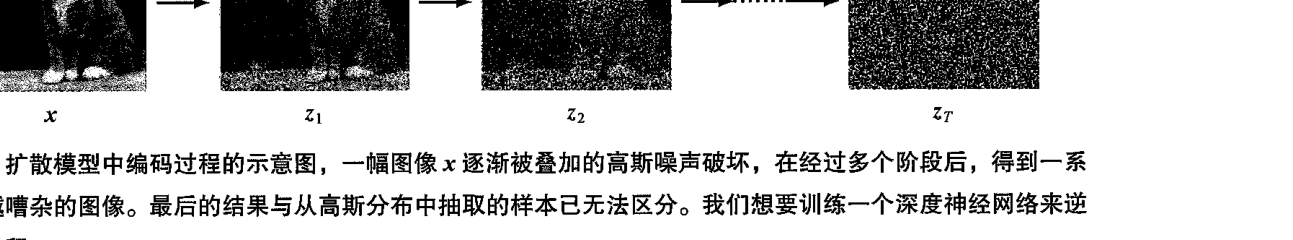
\includegraphics[width=0.9\textwidth]{ch20-fig523-forward.png}
\caption{扩散模型中编码过程的示意图。一幅图像 $x$ 逐渐被叠加的高斯噪声破坏，在经过多个阶段后，得到一系列越来越嘈杂的图像。最后的结果与从高斯分布中抽取的样本已无法区分。我们想要训练一个深度神经网络来逆转这个过程。}
\label{fig:ch20-forward}
\end{figure}

扩散模型可以视为一种层次化的变分自编码器，其中编码器分布是固定的，并由噪声过程定义，只有生成分布是学习得来的（Luo, 2022）（参见 19.2 节）。它们易于训练，在并行硬件上具有良好的可扩展性，在避免对抗训练所带来的挑战和不稳定性的同时，可以产生与生成对抗网络相当或更优的结果。然而，由于需要通过解码器网络进行多次前向传播，它在生成新样本时会产生高昂的计算成本（Dhariwal and Nichol, 2021）。

从训练集中选取一个图像，表示为 $x$，然后将图像中的每个像素独立地与高斯噪声混合，得到一个被噪声损坏的图像 $z_1$，其定义如下：
\begin{align}
z_1=\sqrt{1-\beta_1}\,x+\sqrt{\beta_1}\,\epsilon_1
\label{align:ch20-step1}
\end{align}
其中 $\epsilon_1\sim\mathcal{N}(\epsilon_1\mid 0,I)$ 且 $\beta_1<1$ 是噪声分布的方差。式~\eqref{align:ch20-step1} 中的系数 $\sqrt{1-\beta_1}$ 和 $\sqrt{\beta_1}$ 确保了 $z_1$ 的分布均值比 $x$ 的分布均值更接近于零，且 $z_1$ 的方差比 $x$ 的方差更接近单位矩阵（见习题 20.1）。我们可以将式~\eqref{align:ch20-step1} 写成以下形式（参见习题 20.2）：
\begin{align}
q(z_1\mid x)=\mathcal{N}\big(z_1\mid \sqrt{1-\beta_1}\,x,\,\beta_1 I\big)
\label{align:ch20-qz1}
\end{align}
然后重复这个过程，加入额外的独立高斯噪声，从而生成一系列越来越多的加噪图像 $z_1,\cdots,z_T$。在关于扩散模型的文献中，这些加噪图像或潜变量有时表示为 $x_1,\cdots,x_T$，而观测变量则表示为 $x_0$。在本书中，我们使用 $z$ 来表示潜变量，并使用 $x$ 来表示观测变量。每一个后续图像由下式给出：
\begin{align}
z_t=\sqrt{1-\beta_t}\,z_{t-1}+\sqrt{\beta_t}\,\epsilon_t
\label{align:ch20-step-t}
\end{align}
其中 $\epsilon_t\sim\mathcal{N}(\epsilon_t\mid 0,I)$。同样，我们也可以将式~\eqref{align:ch20-step-t} 写成以下形式：
\begin{align}
q(z_t\mid z_{t-1})=\mathcal{N}\big(z_t\mid \sqrt{1-\beta_t}\,z_{t-1},\,\beta_t I\big)
\label{align:ch20-markov}
\end{align}

条件分布序列 [式~\eqref{align:ch20-markov}] 形成了一条马尔可夫链，并且可以表示为图~\ref{fig:ch20-graphical} 所示的概率图模型（参见 11.3 节）。方差参数 $\beta_t\in(0,1)$，并且通常是手动设置的，它们按预定的计划递增，即 $\beta_1<\beta_2<\cdots<\beta_T$。

\begin{figure}[htbp]
\centering
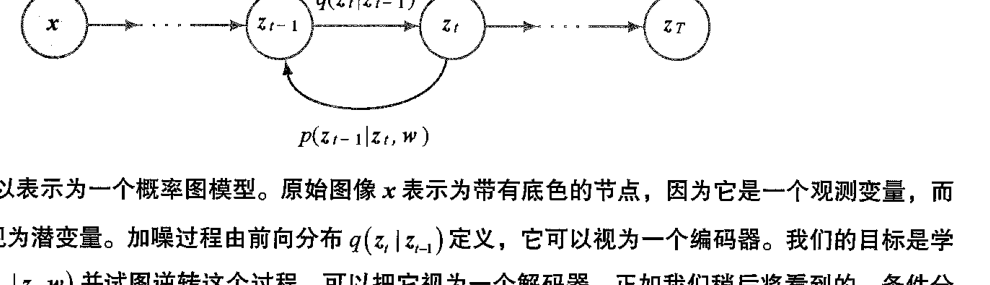
\includegraphics[width=0.85\textwidth]{ch20-fig524-graphical.png}
\caption{扩散过程可以表示为一个概率图模型。原始图像 $x$ 表示为带有底色的节点，因为它是一个观测变量，而加噪图像 $z_1,\cdots,z_T$ 则视为潜变量。加噪过程由前向分布 $q(z_t\mid z_{t-1})$ 定义，它可以视为一个编码器。我们的目标是学习一个条件分布 $p(z_{t-1}\mid z_t,w)$ 并试图逆转这个过程，可以把它视为一个解码器。}
\label{fig:ch20-graphical}
\end{figure}

这个马尔可夫链 [式~\eqref{align:ch20-markov}] 通常称为\textbf{前向过程}（forward process），它类似于 VAE 中的编码器，但这里的马尔可夫链是固定的而不是通过训练得来的。

\subsection{扩散核}\label{subsection:ch20-扩散核}

在观测到数据向量 $x$ 的条件下，潜变量的联合分布由下式给出：
\begin{align}
q(z_1,z_2,\cdots,z_T\mid x)=\prod_{t=1}^{T}q(z_t\mid z_{t-1})
\label{align:ch20-joint}
\end{align}
对中间变量 $z_1,\cdots,z_{T-1}$ 进行边缘化，即可得到\textbf{扩散核}（diffusion kernel）（参见习题 20.3）：
\begin{align}
q(z_t\mid x)=\mathcal{N}\big(z_t\mid \sqrt{\bar{\alpha}_t}\,x,\,(1-\bar{\alpha}_t)I\big)
\label{align:ch20-diffusion-kernel}
\end{align}
其中的 $\bar{\alpha}_t$ 由下式给出：
\begin{align}
\bar{\alpha}_t=\prod_{s=1}^{t}(1-\beta_s)
\label{align:ch20-alpha-bar}
\end{align}

可以看到，每一个中间分布都是一个简单的闭式的高斯分布，我们可以直接从中采样，这在训练 DDPM 时非常有用，因为它允许我们使用马尔可夫链中随机选择的中间项进行高效的随机梯度下降，而不必运行整个马尔可夫链。我们也可以将式~\eqref{align:ch20-step-t} 写成以下形式：
\begin{align}
z_t=\sqrt{\bar{\alpha}_t}\,x+\sqrt{1-\bar{\alpha}_t}\,\epsilon_t
\label{align:ch20-direct-sample}
\end{align}
其中仍然有 $\epsilon_t\sim\mathcal{N}(\epsilon_t\mid 0,I)$。请注意，这里的 $\epsilon_t$ 代表添加到原始图像上的总噪声，而不是在马尔可夫链这一步骤中添加的增量噪声。

在经过多个这样的步骤之后，图像变得与高斯噪声无法区分。在 $T\to\infty$ 的情况下，我们有（见习题 20.4）
\begin{align}
q(z_T\mid x)=\mathcal{N}(z_T\mid 0,I)
\label{align:ch20-asymptotic}
\end{align}
由于式~\eqref{align:ch20-asymptotic} 的右侧独立于 $x$，因此可以得出 $z_T$ 的边缘分布：
\begin{align}
q(z_T)=\mathcal{N}(z_T\mid 0,I)
\label{align:ch20-marginal-t}
\end{align}
因此，关于原始图像的所有信息都丢失了。在式~\eqref{align:ch20-step-t} 中，系数 $\sqrt{1-\beta_t}$ 和 $\sqrt{\beta_t}$ 确保了一旦马尔可夫链收敛到均值为零、协方差为单位矩阵的分布后，就不会再受进一步更新的影响（见习题 20.5）。

\subsection{条件分布}\label{subsection:ch20-条件分布}

我们的目标是学会逆转加噪过程，因此很自然地要考虑条件分布 $q(z_{t-1}\mid z_t)$ 的逆过程，可以使用贝叶斯定理把它表示为
\begin{align}
q(z_{t-1}\mid z_t)=\frac{q(z_t\mid z_{t-1})\,q(z_{t-1})}{q(z_t)}
\label{align:ch20-reverse-bayes}
\end{align}
我们可以将边缘分布 $q(z_t)$ 写成如下形式：
\begin{align}
q(z_t)=\int q(z_t\mid x)\,p(x)\,\mathrm{d}x
\label{align:ch20-marginal-z}
\end{align}
其中 $q(z_t\mid x)$ 由条件高斯分布 [式~\eqref{align:ch20-diffusion-kernel}] 给出。然而，这个分布是难以计算的，因为我们必须对未知的数据密度 $p(x)$ 进行积分。如果我们使用训练集中的样本来近似地进行积分，则会得到一个以高斯函数混合形式表示的复杂分布。

换个思路，考虑逆向分布的条件版本，该分布以数据向量 $x$ 为条件，定义为 $q(z_{t-1}\mid z_t,x)$，这实际上是一个简单的高斯分布。从直观上看这是合理的，因为我们很难猜测哪个低噪声图像演变为某个具体的加噪图像，然而如果我们知道原始图像，那么问题解决起来就会变得容易很多。利用前向过程的马尔可夫性质，可以得到
\begin{align}
q(z_{t-1}\mid z_t,x)=\frac{q(z_t\mid z_{t-1},x)\,q(z_{t-1}\mid x)}{q(z_t\mid x)}
\label{align:ch20-conditional-reverse}
\end{align}

从直观上看，如果我们保持方差较小，使得 $\beta_t$ 远小于 $1$，那么潜向量之间的步骤变化将相对较小，因此学会逆转变换应该更容易。更具体地说，如果 $\beta_t$ 远小于 $1$，那么分布 $q(z_{t-1}\mid z_t)$ 将近似于关于 $z_t$ 的高斯分布。这一点从式~\eqref{align:ch20-reverse-bayes} 中可以看出，因为等式右边是通过 $q(z_t\mid z_{t-1})$ 和 $q(z_{t-1})$ 与 $z_t$ 相关联的。如果 $q(z_t\mid z_{t-1})$ 是一个极其狭窄的高斯分布，那么在 $q(z_{t-1}\mid z_t)$ 具有显著概率质量的区域，$q(z_{t-1})$ 的变化将非常小，因此 $q(z_{t-1}\mid z_t)$ 也可以近似认为是高斯分布。这种直觉可以通过图~\ref{fig:ch20-reverse-approx} 所示的简单例子来证实。然而，由于每一步的方差都很小，我们必须使用大量的步骤来确保从前向加噪过程中获得的最终潜变量 $z_T$ 的分布仍然接近高斯分布，这增加了生成新样本的成本。在实践中，$T$ 的值可能达到数千。

\begin{figure}[htbp]
\centering
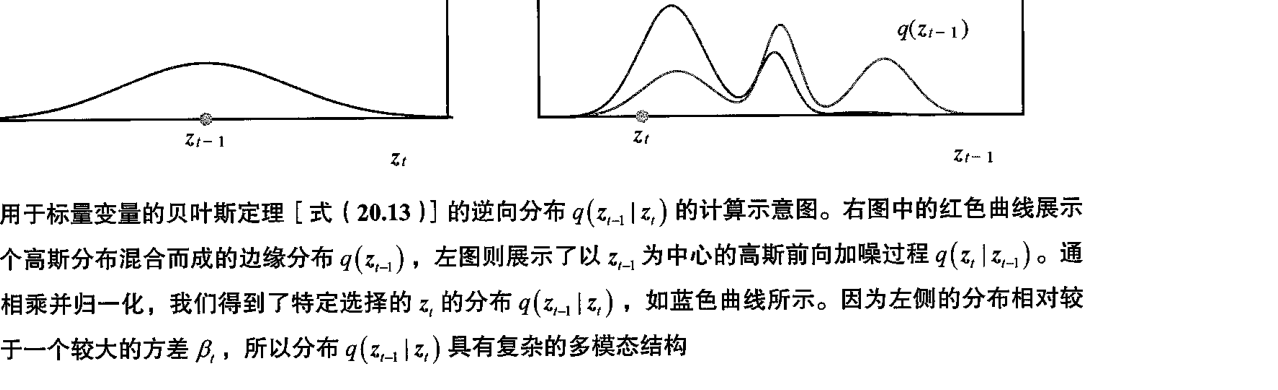
\includegraphics[width=0.85\textwidth]{ch20-fig528-reverse-approx.png}
\caption{用于标量变量的贝叶斯定理 [式~\eqref{align:ch20-reverse-bayes}] 的逆向分布 $q(z_{t-1}\mid z_t)$ 的计算示意图。右图中的红色曲线展示了使用三个高斯分布混合而成的边缘分布 $q(z_{t-1})$；左图则展示了以 $z_t$ 为中心的高斯前向加噪过程 $q(z_t\mid z_{t-1})$。通过将这些相乘并归一化，我们得到了特定选择的 $z_t$ 的分布 $q(z_{t-1}\mid z_t)$，如蓝色曲线所示。因为左侧的分布相对较宽，对应于一个较大的方差 $\beta_t$，所以分布 $q(z_{t-1}\mid z_t)$ 具有复杂的多模态结构。}
\label{fig:ch20-reverse-approx}
\end{figure}

\end{document}